\documentclass[11pt,
  paper=a4, 
  bibliography=totocnumbered,
	captions=tableheading,
	BCOR=10mm
]{scrreprt}

\usepackage[utf8]{inputenc}
 
 
\usepackage[onehalfspacing]{setspace}
\usepackage{csquotes} % Context sensitive quotation.
\usepackage{amsmath} % Standard math.
\usepackage{amsthm} % Math theorems.
\usepackage{amssymb} % More math symbols.
\theoremstyle{definition}
\newtheorem{definition}{Definition}[chapter]
 
\usepackage[section]{placeins} % Keep floats in the section they were defined in.
\usepackage{tabularx}
\usepackage{booktabs} % Scientific table styling.
\usepackage{floatrow} % Option for keeping floats in the place they were defined in the code.
\floatsetup[table]{style=plaintop}
\usepackage{hyperref} % Hyperlinks.
\usepackage[all]{nowidow} % Prevent widows and orphans.
\usepackage{xstring} % logic string operations
\usepackage[nopostdot, nonumberlist]{glossaries} % glossary for definitions and acronyms, without dot after entry and page reference 
\usepackage{bbm} % \mathbb on numerals.
\usepackage{csquotes}
\usepackage{mathtools}
\usepackage[ruled,vlined]{algorithm2e} % Pseudocode
\usepackage{scrhack} % Make warning go away.

\usepackage{graphicx}
\usepackage{subcaption} % Subfigures with subcaptions.
\usepackage{authoraftertitle} % Make author, etc., available after \maketitle
\usepackage{listofitems}
\usepackage{blindtext} % Placeholder text.
\usepackage[nopostdot, nonumberlist]{glossaries}
\makeglossaries % Generate the glossary

% \PassOptionsToPackage{obeyspaces}{url}%
\usepackage[backend=bibtex,% 
style=nature,% 
doi=true,isbn=false,url=false, eprint=false]{biblatex}
% \renewbibmacro*{url}{\printfield{urlraw}}

\addbibresource{bib/library.bib}

\DeclareStyleSourcemap{
  \maps[datatype=bibtex, overwrite=true]{
    \map{
      \step[fieldsource=url, final]
      \step[typesource=misc, typetarget=online]
    }
    \map{
      \step[typesource=misc, typetarget=patent, final]
      \step[fieldsource=institution, final]
      \step[fieldset=holder, origfieldval]
    }
  }
}

%\linespread{1.5} % set line spacing
 
\usepackage{listings} % rendering program code
\lstset{% general command to set parameter(s)
	basicstyle=\ttfamily\color{grey},          % print whole listing small
	keywordstyle=\color{black}\bfseries\underbar,
	% underlined bold black keywords
	identifierstyle=,           % nothing happens
	commentstyle=\color{white}, % white comments
	stringstyle=\ttfamily,      % typewriter type for strings
	showstringspaces=false}     % no special string spaces


\DeclareFontFamily{U}{mathx}{\hyphenchar\font45}
\DeclareFontShape{U}{mathx}{m}{n}{
      <5> <6> <7> <8> <9> <10>
      <10.95> <12> <14.4> <17.28> <20.74> <24.88>
      mathx10
      }{}
\DeclareSymbolFont{mathx}{U}{mathx}{m}{n}
\DeclareFontSubstitution{U}{mathx}{m}{n}
\DeclareMathSymbol{\bigtimes}{1}{mathx}{"91}

 

%%% Custom definitions %%%
% Shorthands
\newcommand{\ie}{i.\,e.~}
\newcommand{\eg}{e.\,g.~}
\newcommand{\ind}{\mathbbm{1}}
% Functions
\newcommand{\tpow}[1]{\cdot 10^{#1}}
\newcommand{\figref}[1]{(Figure \ref{#1})}
\newcommand{\figureref}[1]{Figure \ref{#1}}
\newcommand{\tabref}[1]{(Table \ref{#1})}
\newcommand{\tableref}[1]{Table \ref{#1}}
\newcommand{\secref}[1]{%
	\IfBeginWith{#1}{chap:}{%
		(cf. Chapter \ref{#1})}%
		{(cf. Section \ref{#1})}%
		}
\newcommand{\sectionref}[1]{%
	\IfBeginWith{#1}{chap:}{%
		Chapter \ref{#1}}%
		{\IfBeginWith{#1}{s}{%
			Section \ref{#1}}%
			{[\PackageError{sectionref}{Undefined option to sectionref: #1}{}]}}}
\newcommand{\chapref}[1]{(see chapter \ref{#1})}
\newcommand{\unit}[1]{\,\mathrm{#1}}
\newcommand{\unitfrac}[2]{\,\mathrm{\frac{#1}{#2}}}
\newcommand{\codeil}[1]{\lstinline{#1}}{} % wrapper for preventing syntax highlight error
\newcommand{\techil}[1]{\texttt{#1}}
\newcommand{\Set}[2]{%
  \{\, #1 \mid #2 \, \}%
}
% Line for signature.
\newcommand{\namesigdate}[1][5cm]{%
	\vspace{5cm}
	{\setlength{\parindent}{0cm}
	\begin{minipage}{0.3\textwidth}
		\hrule 
		\vspace{0.5cm}
		{\small city, date}
	\end{minipage}
	 \hfill
	\begin{minipage}{0.3\textwidth}
		\hrule
		\vspace{0.5cm}
	    {\small signature}
	\end{minipage}
	}
}
% Math
\newcommand{\TP}{\text{TP}}
\newcommand{\TN}{\text{TN}}
\newcommand{\FP}{\text{FP}}
\newcommand{\FN}{\text{FN}}

% Automatically use the first sentence in a caption as the short caption.
\newcommand\slcaption[1]{\setsepchar{.}\readlist*\pdots{#1}\caption[{\pdots[1].}]{#1}}

% Variables. 
% Adapt if necessary, use to refer to figures and graphics.
\def \figwidth {0.9\linewidth}
\graphicspath{ {./graphics/figures/}{./graphics/figures/} } % Path to figures and images.


% Customizations of existing commands.
\renewcommand{\vec}[1]{\mathbf{#1}}
% Capitalized \autoref names.
\renewcommand*{\chapterautorefname}{Chapter}
\renewcommand*{\sectionautorefname}{Section}

\DeclareCaptionType{equ}[][]

% TODO Fill with your data.
\title{My full title}
\author{Sven Groen}

\begin{document}

\begin{titlepage}
	\begin{flushleft}
		Universität Osnabrück\\
		Fachbereich Humanwissenschaften\\
		Institute of Cognitive Science
	\end{flushleft}

	\vspace{2cm}
	\centering{
		Bachelorthesis\vspace{1cm}\\
		\textbf{\Large{\MyTitle}}
		\vspace{1cm}\\
		\begin{tabular}{c}
			\MyAuthor                          \\
			970219                            \\
			Bachelor's Program Cognitive Science \\
			Starting month and year - end month and year
		\end{tabular}}
	\vspace{1cm}

	\begin{tabular}{ll}
		First supervisor:  & Dr. Ulf Krumnack          \\
		                   & Institute of Cognitive Science            \\
		                   & Osnabrück                \\\\
		Second supervisor: & Manuel Kolmet         \\
		                   & IMANOX GmbH  \\
		                   & Berlin 
	\end{tabular}

\end{titlepage}


\chapter*{Declaration of Authorship}
I hereby certify that the work presented here is, to the best of my knowledge and belief, original and the result of my own investigations, except as acknowledged, and has not been submitted, either in part or whole, for a degree at this or any other university.

\namesigdate
\pagenumbering{gobble}
\pagebreak

\begin{abstract}
	\textbf{\LARGE{Abstract}}\\\\
	%TODO summarize the main objectives and outcomes of your work. The abstract should fit on one page.
	This is the abstract.
\end{abstract}




%\tableofcontents
%\listoffigures
%\listoftables
%\listofalgorithms


\chapter{Introduction}
\pagenumbering{arabic}
\section{Motivation}
- usually flickering between two frames of the video sequence, 
and ghost objects or partly incorrectly segmented objects often occur only in a single frame, 
while they are classified correctly in the next frame \cite{Pfeuffer2_2019}.

\section{Goal of the thesis}

The goal of this bachelor thesis is to improve the quality of the semantic segmentation of the current IMANOX photo booth using machine learning techniques.
The machine learning model will be an artificial neural network architectures covered in section \ref{sec:related_work}.
This model will be altered and changed towards the needs of the project and will be trained with custom training data.
It will be investigated whether additional temporal information leads to an improvement of the already existing segmentation models (see Section \ref{ch:Methods}).
When looking at successful semantic segmentation models, it can be noticed that the prediction occurs on bases of individual images.
It can be argued that in \textit{real world scenarios} a semantic segmentation on single images is not as required as it is on videos, which are streams of frames.
Potential applications include autonomous driving or video effects in the film industry.


When working with video data, valuable temporal information might get lost when the segmentation occurs on individual frame level.
Therefore, the thesis will investigate whether the temporal information that is present in video data can be used for improvement of performance by adding recurrent structures
into existing semantic segmentation models. 
Given the collaboration with IMANOX and their goal to replace their \textit{virtual background change}-technique, the focus of the thesis will be on binary semantic segmentation
instead of the typical multiclass segmentation. 

\section{Semantic Segmentation}

\textcite{Szeliski2011} refers to image segmentation as "the task of finding groups of pixels that 'go together'" (\cite{Szeliski2011}, p. 237).
How the pixels are \textit{grouped together} can be achieved in different ways.
In the classical image classification tasks, the task is to simply name the objects that can be seen in an image.
Semantic image segmentation extends this problem further, referring to a pixel-wise classification of an image \cite{Minaee2020}.
Each pixel in an image is assigned to one category label given a set of categories.
However, individual instances of an object in one image are not differentiated but labeled as one class.
Instance segmentation combines a pixel-wise classification (similar to semantic segmentation) with an additional object detection and localization, differentiating each individual instance of a class \cite{Minaee2020}.
Given the goal of this project, only binary semantic segmentation is necessary.
Detailed information about which objects are in the scene is not required.
\begin{figure}[H]
	\centering
	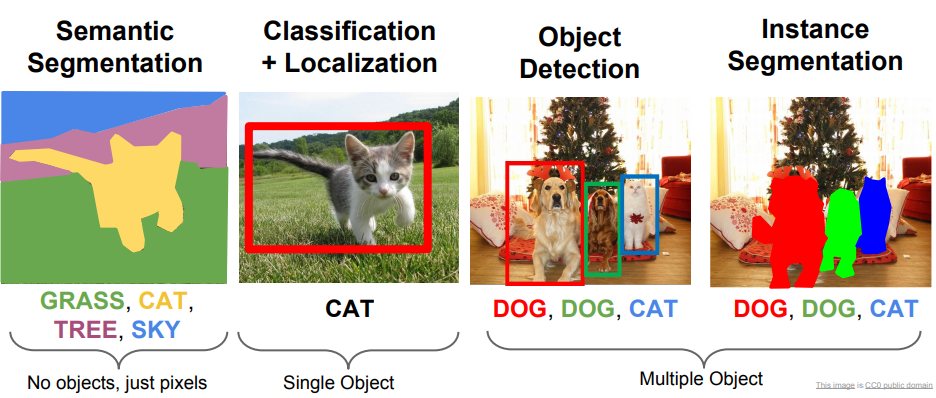
\includegraphics[width=\figwidth]{Computer_Vision_Tasks}
	\slcaption{
		Overview of Computer Vision Tasks. (\textcite{Fei-Fei2017}, Slide 17).
		\label{fig:Computer_Vision_Tasks}}
\end{figure}


\section{Recurrent Neural Networks} \label{ch:RNN}

Recurrent Neural Networks (RNNs) are a special kind of artificial neural network that is able to process sequential data \cite{Valipour2017, Sherstinsky2020} and "extract temporal dependencies" \cite{Hochreiter1998}.
In Sequential data the order of the data is of importance and therefore carries information, for example speech recognition or time variant problems \cite{Hoffmann2017, Pfeuffer2_2019}.
RNNs contain a hidden recurrent state, which enables them to process sequential data \cite{Hoffmann2017, Valipour2017}.
Although they have been applied succesfully to many problems in the sequential data domain \cite{Sherstinsky2020}, they are often criticized for their computational complexity due to their recurrent structure \cite{Pfeuffer2_2019}.
They are also known for struggling in learning long term dependencies \cite{Hoffmann2017}.

The reason for this is the vanishing- and exploding gradient effect \cite{Hochreiter1998}.
\textcite{Hochreiter1991} was the first to identified the vanishing gradient effect \cite{Skansi2018}.
The gradient of the loss is used to update the models weights during the backpropagation, enabling the \textit{learning} of the model \cite{Suzuki2017, Skansi2018}.
The gradient of early layers of deep networks dependent on the gradient of later layers because the gradient is propagated backwards through the network \cite{Skansi2018}.
For recurrent neural networks this backpropagation of the gradient is called \textit{backpropagation through time} (BPTT) \figref{fig:rnn-bptt-with-gradients}, 
where the gradient for any time step is dependent on all previous timesteps \cite{Skansi2018}.


\begin{figure}[H]
	\centering
	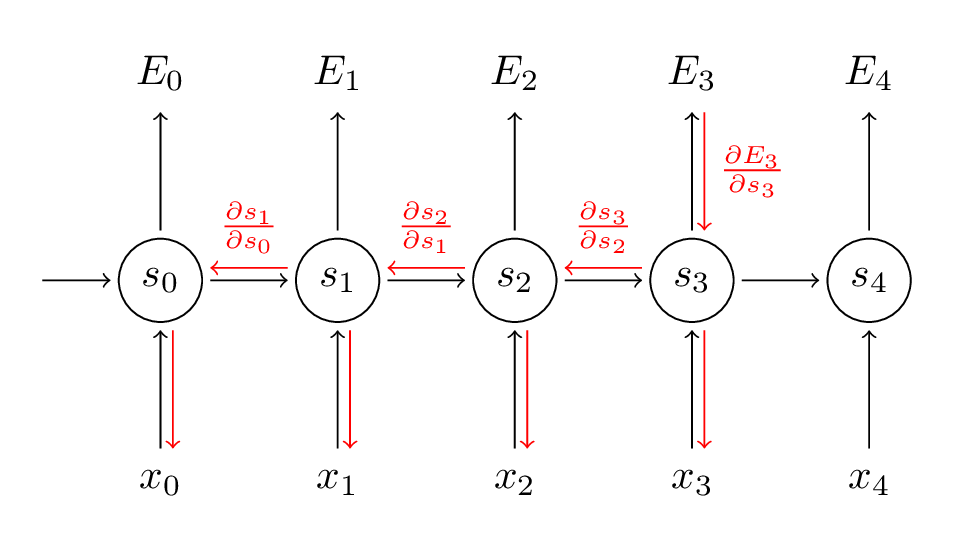
\includegraphics[width=\figwidth]{rnn-bptt-with-gradients}
	\slcaption{
		backpropagation through time (\textcite{Britz2015}).
		\label{fig:rnn-bptt-with-gradients}}
\end{figure}

The \textit{vanishing gradient effect} occurs since derivatives are repeatedly multiplied \cite{Skansi2018}. 
If a gradient is zero or close to zero the amount of learning in the previous layers is very small, 
since their gradient is very small due to their predecessors being very small \cite{Britz2015, Hochreiter1991}.
\textcite{Pascanu2013} states that the \textit{vanishing gradient effect} occurs 
"when long term components go exponentially fast to norm 0, 
making it impossible for the model to learn correlation between temporally distant events."

During an explosion of long term dependencies the \textit{exploding gradient effect} occurs \cite{Pascanu2013}.
Here, during backpropagation the gradient can can grow exponentially with each layer \cite{Philipp2017, Hochreiter1997}.
The \textit{learning step} would simply be to large, leading the model not closer to an optimum but further away \cite{Skansi2018}.


\subsection{Long-Short-Term-Memory} \label{sec:LSTM}
The Long Short Term Memory (LSTMs) networks by \textcite{Hochreiter1997} tackles the problem of vanishing and exploding gradient successfully \cite{Skansi2018}.
They are categorized as a special kind of RNNs \cite{Hoffmann2017}, made up of several gates \figref{fig:LSTM-chain} which control how information flows through the network \cite{Valipour2017}.
There is an input gate, a forget gate and an output gate which are able to learn \cite{Valipour2017} and control what information is removed an what information is added \cite{Skansi2018}.
This way LSTMs are able to learn to detect \textit{long term dependencies} \cite{Chung2014}.

\begin{figure}[H]
	\centering
	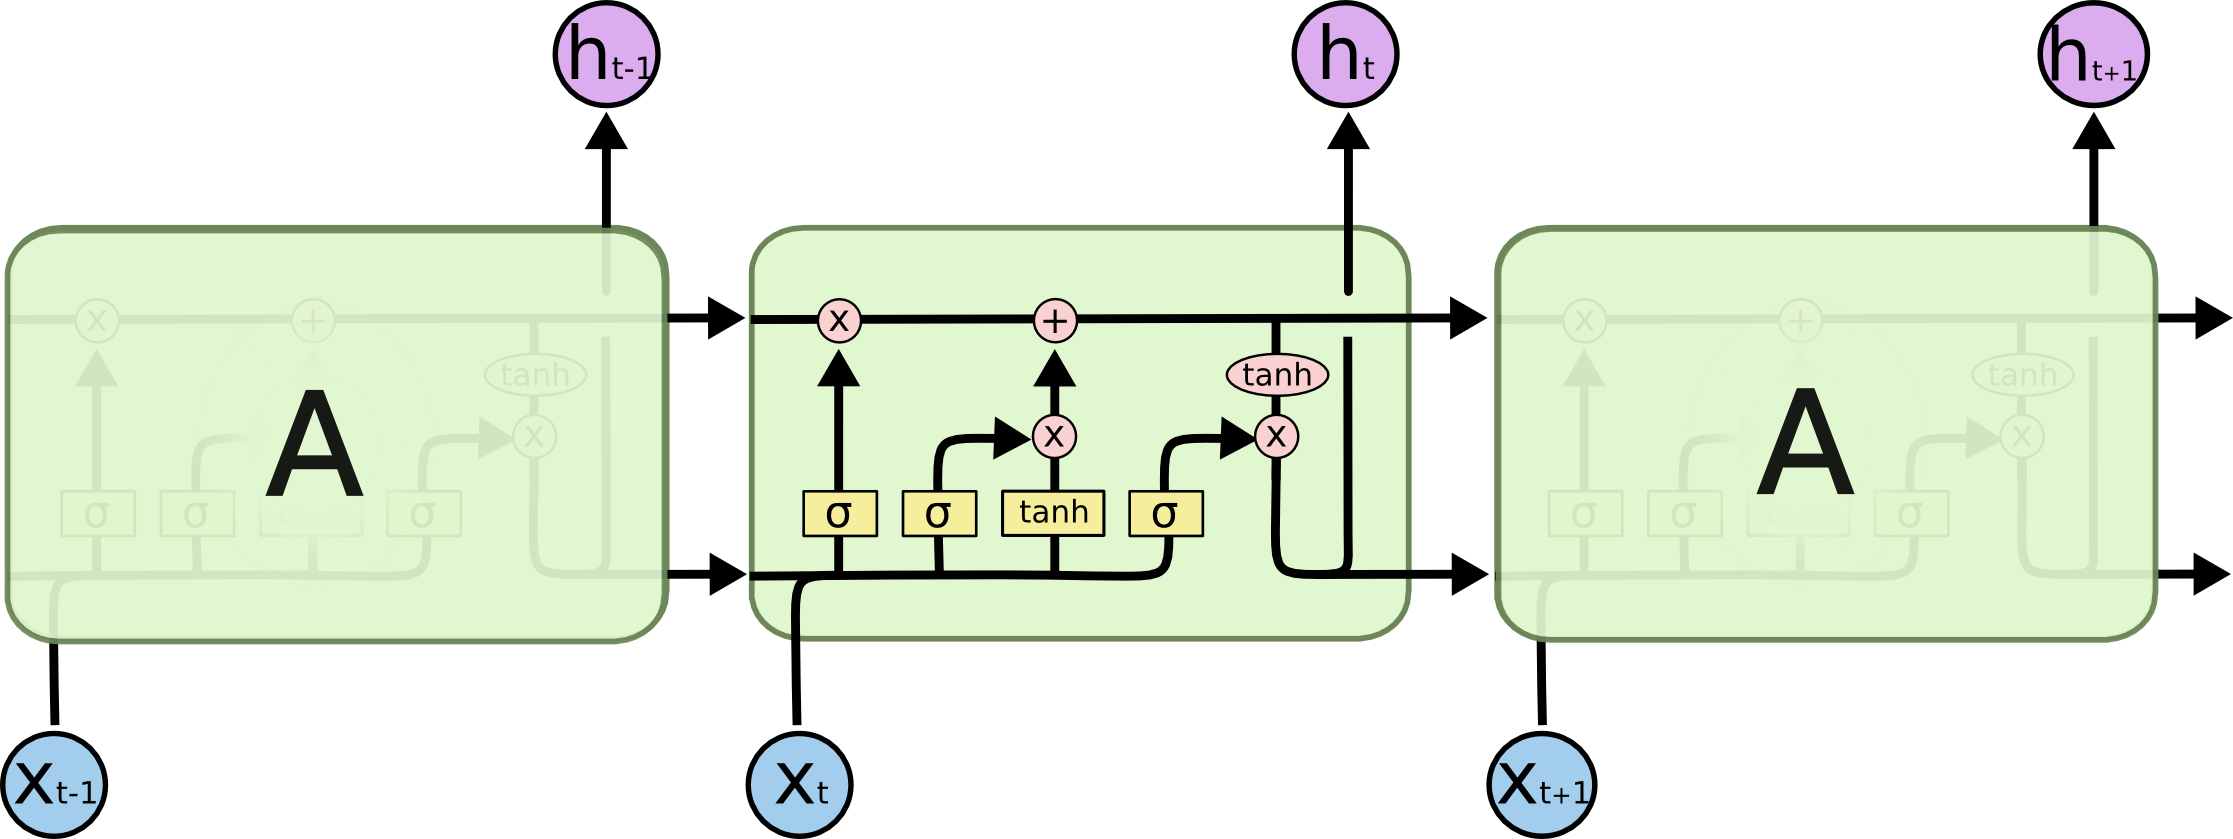
\includegraphics[width=\figwidth]{LSTM-chain}
	\slcaption{
		Long-Short-Term-Memory Architecture (\textcite{Olah2015}).
		\label{fig:LSTM-chain}}
\end{figure}

\begin{equ}[!ht]
	\begin{equation}
		f_t = \sigma{(W_f * [h_{t-1},x_t] + b_f)} % Concatination?
	\end{equation}
	\begin{equation}
		i_t = \sigma{(W_i * [h_{t-1},x_t] + b_i)}
	\end{equation}
	\begin{equation}
		o_t = \sigma{(W_o * [h_{t-1},x_t] + b_o)}
	\end{equation}
	\begin{equation}
		\widetilde{C}_t = \tanh{(W_C * [h_{t-1},x_t] + b_C)} 
	\end{equation}
	\begin{equation}
		C_t= f_t * C_{t-1} + i_t * \widetilde{C}_t 
	\end{equation}
	\begin{equation}
		h_t = o_t * \tanh{(C_t)}
	\end{equation} 
\caption{Formulas to compute the different gates and states. Extracted from \textcite{Olah2015} and \textcite{Chung2014}} %Nummerierung stimmt nicht (1.1)
\end{equ}

The LSTM network has in addition to the hidden state a so called a "memory cell" \cite{Hochreiter1997} or "cell (internal) state" \cite{Valipour2017, Skansi2018,Olah2015, Yurdakul2017}
$f_t$ denotes the output of the "forget gate", which is calculated by the hidden state from the previous timestep ($h_{t-1}$) and the current input $x_t$ at time point $t$ \cite{Olah2015}.
It controls how much of the input and the hidden state should be remembered \cite{Skansi2018}.
$i_t$ refers to the output of the "input gate", which purpose is "to protect the memory contents stored (...) from perturbation by irrelevant inputs" \cite{Hochreiter1997}.
"Candidate values" \cite{Olah2015} $\widetilde{C}_t$ are calculated and are combined with $i_t$ to update the cell state $C_t$ \cite{Hochreiter1997}.
The cell state $C_t$ is updated with each new input by the result of the forget gate $f_t$ and the result of $i_t * \widetilde{C}_t$ \cite{Chung2014}.
The different gates can be seen as \textit{filters} that determine which information will be saved in the cell state \cite{Skansi2018}.
Finally, the new hidden state $h_t$ is based on the result of the output gate $o_t$ combined with the new resulting cell state $C_t$.

As previously stated, vanilla LSTM are capable to process one dimensional sequential data through several gates and operations.
\textcite{Shi2015} proposed an extension of the fully connected LSTM by replacing multiplication operations by convolution operations called \textit{Convolutional LSTM} (ConvLSTM)\cite{Yurdakul2017, Nabavi2018}.
This way the spatial information that might be incorporated in the data (\eg images) will not get lost through any kind of dimension reduction that would have been necessary previously \cite{Shi2015}.
Their biggest advantage is they are able to keep the dimensions of the input while reducing the necessary parameters \cite{Pfeuffer2_2019}.
Further research towards improving the ConvLSTM architecture has been done.
\textcite{Pfeuffer2_2019} proposed three alternations, namely \textit{Spatially Separable- , Depthwise- and Depthwise Separable Convolutional LSTMs}, 
which reduced the number of parameters and operations while keeping a comparable performance like the original ConvLSTM \cite{Pfeuffer2_2019}.

\subsection{Gated-Recurrent-Unit} \label{sec:GRU}
\textcite{Cho2014} proposed an alternative architecture that is able to learn long term dependencies using gates \cite{Chung2014}, the \textit{Gated Recurrent Unit} (GRU).
The GRU architecture is similar to the LSTM architecture, but reduces the number of gates from three to two, namely and \textit{update-} $z_t$ and a \textit{reset gate} $r_t$ \cite{Dey2017}.
Moreover, the memory cell that was present in the LSTM is merged with the hidden state in the GRU \cite{Olah2015}.
The output flow of information is not controlled by the output gate anymore but is determined indirectly by the update- and reset gate that control the information of the hidden state \cite{Siam2018}

\begin{equ}[!ht]
	\begin{equation}
		z_t = \sigma{(W_z * [h_{t-1},x_t])} % Concatination?
	\end{equation}
	\begin{equation}
		r_t = \sigma{(W_r * [h_{t-1},x_t])}
	\end{equation}
	\begin{equation}
		\widetilde{h}_t = \tanh{(W * [r_t*h_{t-1},x_t])} 
	\end{equation}
	\begin{equation}
		h_t = (1-z_t)*h_{t-1}+z_t*\widetilde{h}_t
	\end{equation} 
\caption{Formulas to compute the different gates and states. Extracted from \textcite{Olah2015} and \textcite{Chung2014}} %Nummerierung stimmt nicht (1.1)
\end{equ}

Less gates than modulate the information flow in fewer states \cite{Chung2014} leads to simpler architecture that is faster to train \cite{Yurdakul2017}
and less memory consuming \cite{Valipour2017}.
While both, LSTMs and GRUs, outperform classical RNNs in task that require long-term dependencies \cite{Chung2014}, GRUs show a similar good performance to the LSTM architecture while having a reduced complexity \cite{Valipour2017}.
\textcite{Dey2017} argues, that GRUs outperform LSTMs in most cases. 
\textcite{Jozefowicz2015} confirms this observation with the restriction that LSTMs outperform GRUs in language modelling tasks.
Research towards reducing the complexity of GRUs is done \cite{Dey2017}.

In order to process two-dimensional data like images, convolutional GRUs (ConvGRUs) have been designed \cite{Ballas2016,Siam2018}.
Dot product operations in the classical GRU are replaced by two dimensional convolution operations \cite{Siam2018} and states and gates are three dimensional tensors \cite{Tokmakov2017}.




\section{Related Work} \label{sec:related_work}


\subsection{Semantic Segmentation}

Segmenting an image into its individual parts is a classical problem of computer vision \cite{Szeliski2011}. 
Early approaches involve typical methods like threshold detection \cite{Smith1979}.
More modern approaches like k-means clustering \cite{Dhanachandra2015} improved the early results.
Deep learning architectures, especially convolutional neural networks (CNNs) \cite{Fukushima1980}, have lead to further improvement.
\textcite{Shelhamer2017} have been the first to propose a CNN architecture where a pixel-wise supervised training was achieved. 
This was done by upsampling the class prediction layer to the input image size, leading to an end to end pixel-wise classification, a \textit{Fully Convolutional Network} (FCN) \cite{Shelhamer2017}.
Following papers proposed different architectures.
A \textit{Deconvolutional Network} with special unpooling and deconvolution operations was invented by \textcite{Noh2015}. 
Here, the information was enconded using several convolutions and poolings and was decoded using unpooling and deconvolution.
The SegNet model uses a similar Encoder-Decoder architecture by using pooling indices to upsample the image \cite{Badrinarayanan2017}.
ICNet \cite{Zhao2017} was able to perform semantic segmentation not only in real-time, but also for high quality images (1024x2048 at 30 fps). 
This was achieved by using a cascade image input of different resolutions. 
The authors made use of the semantic information from the scaled down images and the details from the high resolution images.
In this way, they have been able to achieve a "trade-off between efficiency and accuracy" (\cite{Zhao2017}, p.2).
Google's approach towards instance segmentation is called Deeplab and has evolved over the last recent years.
The first DeepLab version uses a combination of Deep CNNs with fully connected conditional random fields (CRFs) that tries to grasp the semantic context of the image \cite{Chen2016}. 
One of their main contributions is the use of atrous (or dilated) convolutions as an alternative to deconvolution. 
Originally used for wavelet transformations, a new parameter r allows to change the stride at which the samples are taken during the convolution operation \cite{Chen2016}.
Applying dilatation during convolution allows to increase the receptive field while keeping the computational costs low \cite{Minaee2020}.
This approach has been further improved and Atrous Spatial Pyramid Pooling (ASPP) \figref{fig:ASPP} has been introduced, which was based on the idea of combining atrous convolutions with spatial pyramid pooling (firstly introduced by \textcite{He2014}) \cite{Chen2018}.

\begin{figure}[H]
	\centering
	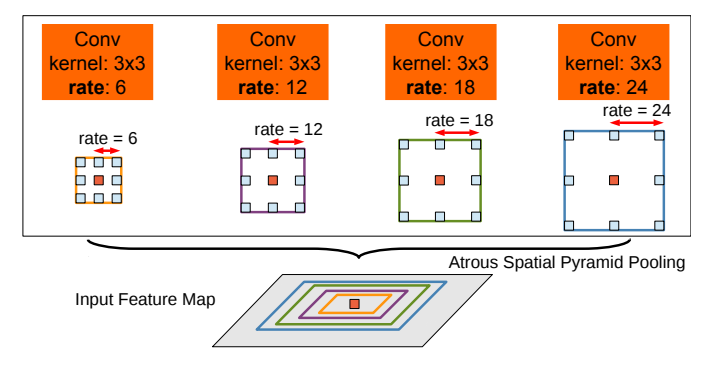
\includegraphics[width=\figwidth]{ASPP}
	\slcaption{
		Atrous Spatial Pyramid Pooling. (\cite{Chen2018a}, Fig. 4).
		\label{fig:ASPP}}
\end{figure}


In ASPP, parallel filters of different dilation rates are concatenated with the intend to cover different field-of-views \cite{Chen2018}, allowing robust object segmentation on different scales \cite{Minaee2020}.
The most recent approach, DeepLab V3+, has an Encoder-Decoder structure and was able to show "new state-of-the-art performance on PASCAL VOC 2012 and Cityscapes datasets." (\cite{Chen2018b}, p.14).
The encoder is based on their previous DeepLabV3 architecture with a modified Xception backbone \cite{Minaee2020}.
The newly introduced decoder is responsible for upsampling the output to the desired size.
This is achieved by concatenating the encoders output with the images \textit{low-level Features} (which are the result of atrous convolutions) and bilinear upsampling, see figure \ref{fig:DLPlus} for the detailed architecture \cite{Chen2018b}.
Moreover, the Google research team has shown that they are able to create an Encoder-Decoder architecture that is very light and fast.
This architecture is light enough to run at real-time on modern smartphones \cite{Bazarevsky2018}.

\begin{figure}[H]
	\centering
	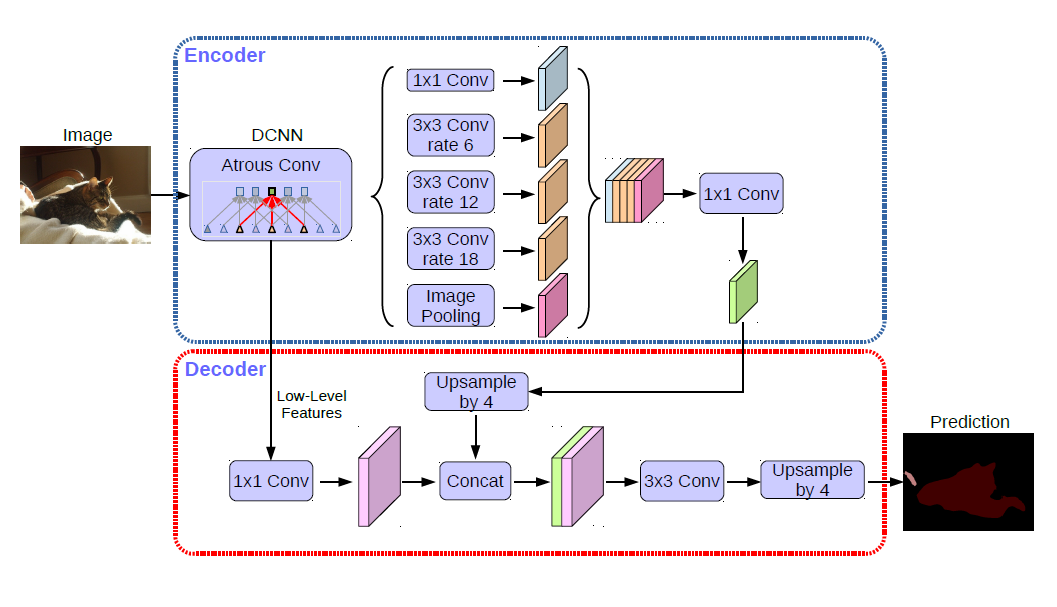
\includegraphics[width=\figwidth]{DLV3Plus}
	\slcaption{
		DeepLabV3+ Encoder-Decoder Architecture. (\cite{Chen2018b}, Fig. 2).
		\label{fig:DLPlus}}
\end{figure}



\subsection{Video processing}

Most of the models are usually evaluated on individual images.
However, in real world scenarios segmentation is often necessary for videos and not just single images.
Naturally, the segmentation works on each individual frame but this way the context of the videos gets lost.
The model is not able to know that the previous frame is related to the current one, it treats each frame independently \cite{Pfeuffer2019}.

Extending existing models with a recurrent unit could enable the model to not only use spatial but also spatiotemporal information\cite{Pfeuffer2019}.
Recurrent neural networks \secref{ch:RNN} are usually the answer to time dependent problems \cite{Hoffmann2017} or used for sequential data such as in time series analysis or text translation. 
\textcite{Valipour2017} was one of the first to introduce a recurrent unit into a segmentation model \cite{Pfeuffer2019}, increasing the models performance by 3 - 5\%.
\textcite{Visin2015} introduced ReSeg, a segmentation model consisting of four RNN layers that "sweep the image horizontally and vertically".
\textcite{Yurdakul2017} was also able to improve performance by incorporating ConvLSTMs (\ref{sec:LSTM}) and ConvGRUs (\ref{sec:GRU}) in their architecture.
% positions of the RU
The positioning of the recurrent unit in the existing models varies across the literature.
\textcite{Pfeuffer2019} notes that recurrent units are often placed in between of the encoder and decoder, such as in \cite{Valipour2017,Yurdakul2017}.
They investigated the effect of the placement of a ConvLSTM cell on the performance of the model and observed that the best position for ConvLSTM layer seems to be directly in front of the last activation layer and not in between the encoder and decoder \cite{Pfeuffer2019}.
In their follow up work \cite{Pfeuffer2_2019}, different ConvLSTM variations have been investigated with the intend to lower the complexity and allow for faster video segmentation.

\subsubsection{real time segmentation}
--> bestehende architectures einfacher/leichter machen

\chapter{Methods} 
\label{ch:Methods}


\section{The Dataset}
\subsection{Requirements}\label{sec:Requirements}
The task of binary semantic segmentation with one foreground and one background task in this work is not a unique one, however, the given detailed context of the task upholds certain requirements towards the dataset that is used for training.
The dataset should have two classes, one foreground and one background class.
The model input images should be in a typicial 3-channel format with Red-Green-Blue (RGB) values in the range of 0 to 255. 
The ground truth the model should try to predict needs to be in a typical 1-channel greyscale format where each pixel is either black or white, representing the background and foreground class respectively.
Since the model is supposed to use temporal information through a RU, the images need to be the individual frames from a video file.
The content of the video should be focused around human beings in the foreground, since the use case scenario of the network is a background replacement task of humans in a convention/event scenario.
In addition to that, it would be usefull if the dataset would be flexible in terms of the background.
As mentioned the backgrounds in the input image that the model is supposed to remove are designed based on the customer.
The specific design is known prior to the models use, which means the dataset should support the possibility to train the model for a specific background in order to improve and overfit the model to some extend towards certain prior given backgrounds.

The final dataset is seperated into a training and testing set.
The training set consist of _____ images and labels while the testing dataset consist of _____ images and labels, corresponding to a ___ to ___ train-test-ratio.

\subsection{Creating the Dataset}
These requirements are very specific and to the best of the authors knowledge, there is no dataset that would fullfill the given requirements.
Therefore, this thesis proposes a newly crafted dataset that is able to fullfill all requirements described in \ref{sec:Requirements}.
The ground truth (GT) images (or \textit{labels}) based on the video input frames are produces in an automatic manner (see \ref{sec:Preprocessing} for details) using a colour threshold algorithm.
Creating high quality GT images by hand is a very laborious work and simply too time consuming considering that individual video frames need to be labeled.
A selection of ___  publicly available greenscreen stock video clips, varying in length from ___ to ___ seconds, is used as the basis for the dataset.
The background of those clips is replaced by one of ____ background images.
The selection of the background images is based on certain criteria that have been made.
Looking at various existing background walls that are used by companies for presentation on conventions one can observe that their designs are usally quite similar.
The overall design is centered around the product of the companies logo and kept very minimalistic with some basic geometric shapes, abstract with some chaotic or repetitive patterns or has a nature like theme.
Based on these criteria the selection of background images for training has been made.

\section{Preprocessing}\label{sec:Preprocessing}
Several preprocessing steps have been done to prepare the data into a format suitable for training.
The raw greenscreen video clips are seperated into four second snippets and scaled down to a resolution of 270x512 pixels.
The resulting clips are randomly shuffled and the green background is replaced one randomly selected background image out of the pool of background images for each of the four second clips.
In order to prevent potential overfitting


\section{Network Architecture}
\section{Training}

\section{Metrics}

In order to evaluate the different models properly objective meassurements are required that allow for a fair comparison across multiple models \cite{Garcia-Garcia2018}. 
\textcite{Minaee2020} and \textcite{Garcia-Garcia2018} nicely summarize the most common metrices used for semantic segmentation.
The \textbf{Pixel accuracy} is defined as the ratio of correctly classified pixels to the total number of pixels:
In our binary context, \textit{True Positives} (TP) denotes the pixels correctly classified as foreground, 
\textit{True Negatives} (TN) denotes the pixels correctly classified as background, 
\textit{False Negatives} (FN) denotes the pixels that are classified as background while actually belonging to the forground class and lastly
\textit{False Positives} (FP) denotes the pixels that are classified as foreground while actually belonging to the background class.


\begin{equation}
	\text{PA} = \frac{(\TP + \TN)}{(\TP + \TN + \FP + \FN)}
\end{equation}

In a more general context, for $k + 1$ classes and pixel $p_{ij}$ denoting the pixel of class i classified as belonging to class j, the pixel accuracy can be described as \cite{Garcia-Garcia2018}:

\begin{equation}
	\text{PA} = \frac{\sum_{i=0}^{k}p_{ii}}{\sum_{i=0}^{k}\sum_{j=0}^{k}p_{ij}}
\end{equation}

The \textbf{Mean Pixel Accuracy} calculates the pixel accuracy for each class and avereges over the total number of classes:

\begin{equation}
	\text{MPA} = \frac{1}{k+1}\sum_{i=0}^{k}\frac{p_{ii}}{\sum_{j=0}^{k}p_{ij}}
\end{equation}


The most frequently used metric in semantic segmentation is the \textbf{Intersection over Union (IoU)} (or \textbf{Jaccard Index}) \cite{Minaee2020}.
It computes the area of overlap of the ground truth and the prediction divided by the union of both areas \cite{Garcia-Garcia2018}:

\begin{equation}
	\text{IoU} = \frac{\TP}{(\TP + \FP + \FN)}
\end{equation}


The \textbf{Mean Intersection over Union (MIoU)} computes the average of the per class calculated IoU's \cite{Garcia-Garcia2018}:

\begin{equation}
	\text{MIoU} = \frac{1}{k+1} \sum_{i=0}^{k} \frac{p_{ii}}{\sum_{j=0}^{k} p_{ij} + \sum_{j=0}^{k} p_{ji}-p_{ii}}
\end{equation}

Lastly, a popular metric is the \textbf{Dice Score}, which is in our boolean context equivialent to the \textbf{F1 score} \cite{Minaee2020}. It is defined as:

\begin{equation}
	\text{Dice}=\frac{2\TP}{2 \TP + \FP+ \FN}
\end{equation}

\chapter{Results}
\chapter{Evaluation and Discussion}
\chapter{Conclusion}


\chapter*{Acknowledgements}
%TODO A place to say thank you to everybody who helped you.


% Acronym definitions
%TODO Add acronym definitions produced by acronyms2glossary.py 




\glsaddall
\printglossaries

\printbibliography

\end{document}